\usepgfplotslibrary{groupplots}


\begin{figure}[!ht]
    \centering
    
    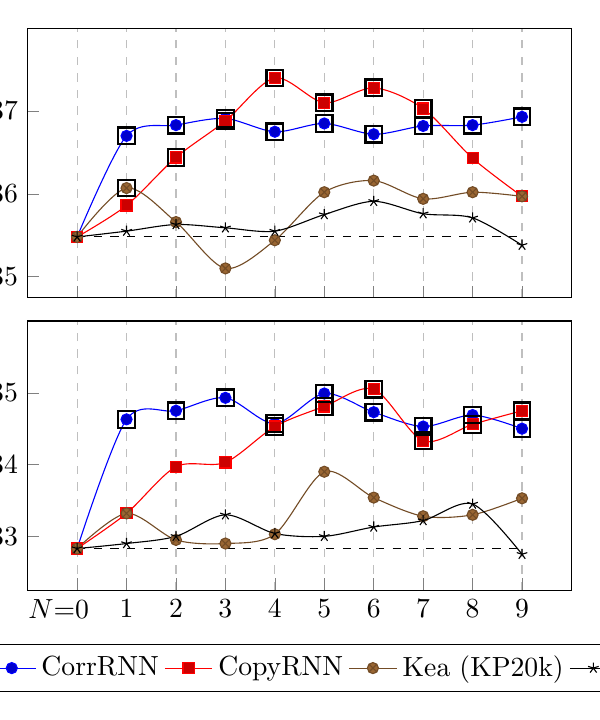
\begin{tikzpicture}[trim axis left,trim axis right]

    \begin{groupplot}[
        group style={
          group size=1 by 2,
          vertical sep=1.3cm,
        },
        width=0.7\textwidth, height=5cm,
        xmin=-1, xmax=10,
        xtick = {0, 1, 2, 3, 4, 5, 6, 7, 8, 9},
        tick pos=left,
        grid style={dashed, gray!50},
        xmajorgrids,
        legend columns=-1,
        legend style={
            anchor=north west,
            at={(-0.09,-0.2)}
        },
    ]
    
    \nextgroupplot[
        ymin=34.75, ymax=38,
        xticklabels={,,,},
        ytick = {35, 36, 37},
    ]
    \node[] at (axis cs: .4, 37.5) {{{{\small \trm}}}};

    \addplot+[smooth] plot coordinates {
        (0, 35.48) (1, 36.70) (2, 36.83) (3, 36.91) (4, 36.75) (5, 36.85) (6, 36.72) (7, 36.82) (8, 36.83) (9, 36.93)};
    \addlegendentry{CorrRNN}
    
    \addplot+[smooth] plot coordinates {
        (0, 35.48) (1, 35.86) (2, 36.44) (3, 36.88) (4, 37.40) (5, 37.10) (6, 37.28) (7, 37.03) (8, 36.43) (9, 35.97)};
    \addlegendentry{CopyRNN}

    \addplot+[smooth] plot coordinates {
        (0, 35.48) (1, 36.07) (2, 35.66) (3, 35.10) (4, 35.44) (5, 36.02) (6, 36.16) (7, 35.94) (8, 36.02) (9, 35.97)};
    \addlegendentry{Kea (KP20k)}

    \addplot+[smooth] plot coordinates {
        (0, 35.48) (1, 35.55) (2, 35.63) (3, 35.59) (4, 35.55) (5, 35.75) (6, 35.91) (7, 35.76) (8, 35.71) (9, 35.38)};
    \addlegendentry{MPRank}

    % baseline
    \addplot[mark=none, black, dashed] coordinates {(0, 35.48) (9, 35.48)};

    % significative points
    \addplot[only marks, mark=square, color=black, thick, mark size=3pt] plot coordinates {
        (2, 36.44) (3, 36.88) (4, 37.40) (5, 37.10) (6, 37.28) (7, 37.03) (1, 36.70) (2, 36.83) (3, 36.91) (4, 36.75) (5, 36.85) (6, 36.72) (7, 36.82) (8, 36.83) (9, 36.93) (1, 36.07)};
    \legend{}

    \nextgroupplot[
        yshift=1cm,
        ymin=32.25,ymax=36,
        xticklabels={$N$=0\quad~~,1, 2, 3, 4, 5, 6, 7, 8, 9},
        ytick = {32, 33, 34, 35},
    ]
    \node[] at (axis cs: .4, 35.5) {{{{\small \tr}}}};
    
    \addplot+[smooth] plot coordinates {
        (0, 32.83) (1, 34.63) (2, 34.75) (3, 34.93) (4, 34.57) (5, 34.99) (6, 34.73) (7, 34.53) (8, 34.69) (9, 34.50)};
    \addlegendentry{CorrRNN}
    
    \addplot+[smooth] plot coordinates {
        (0, 32.83) (1, 33.32) (2, 33.97) (3, 34.03) (4, 34.53) (5, 34.81) (6, 35.05) (7, 34.33) (8, 34.56) (9, 34.75)};
    \addlegendentry{CopyRNN}
    
    \addplot+[smooth] plot coordinates {
        (0, 32.83) (1, 33.32) (2, 32.95) (3, 32.90) (4, 33.03) (5, 33.90) (6, 33.54) (7, 33.28) (8, 33.30) (9, 33.53)};
    \addlegendentry{Kea (KP20k)}
    
    
    \addplot+[smooth] plot coordinates {
        (0, 32.83) (1, 32.90) (2, 33.00) (3, 33.30) (4, 33.04) (5, 33.00) (6, 33.13) (7, 33.22) (8, 33.45) (9, 32.75)};
    \addlegendentry{MPRank}
    
    
    % baseline
    \addplot[mark=none, black, dashed] coordinates {(0, 32.83) (9, 32.83)};
    
    % significative points
    \addplot[only marks, mark=square, color=black, thick, mark size=3pt] plot coordinates {
        (4, 34.53) (5, 34.81) (6, 35.05) (7, 34.33) (8, 34.56) (9, 34.75) (1, 34.63) (2, 34.75) (3, 34.93) (4, 34.57) (5, 34.99) (6, 34.73) (7, 34.53) (8, 34.69) (9, 34.50)};

    \end{groupplot}
    %\end{axis}
    
    \end{tikzpicture}
    %\end{subfigure}


    \caption{Scores de \map{} pour \textsc{Bm25}+RM3 sur NTCIR-2 en fonction du nombre $N$ de mots-clés prédits. Le symbole $\square$ indique une amélioration significative par rapport aux résultats sans mots-clés prédits.}
    \label{fig:n_vs_perf}
\end{figure}